%!TeX program = xelatex
\documentclass[12pt,hyperref,a4paper,UTF8]{ctexart}
\usepackage{SJTUReport}
\usepackage{float}
\usepackage{graphicx}
\usepackage{subfigure}
\usepackage{parskip}
\usepackage{booktabs}
%%-------------------------------正文开始---------------------------%%
\begin{document}

%%-----------------------封面--------------------%%
\cover

%%------------------摘要-------------%%
%\begin{abstract}
%
%在此填写摘要内容
%
%\end{abstract}

\thispagestyle{empty} % 首页不显示页码

%%--------------------------目录页------------------------%%
\newpage
\tableofcontents

%%------------------------正文页从这里开始-------------------%
\newpage

%%可选择这里也放一个标题
%\begin{center}
%    \title{ \Huge \textbf{{标题}}}
%\end{center}

\noindent \textbf{摘要:}维生素C是人体营养中最重要的维生素之一,主要存在于新鲜水果及蔬菜中,适当补充维生素C可以有效预防动脉粥样硬化等心血管疾病。本实验以柑橘为原材料,采用滴定法对比研究不同温度条件对橘子中维生素C热稳定性的影响。结果表明,随着温度升高,柑橘中的维生素C含量会不断减少。\\

\textbf{关键字:}维生素C;2,6-二氯酚靛酚;温度;滴定;热稳定性
\section{前言}
维生素C,是一种多羟基化合物,结构类似葡萄糖,其分子极易解离而释放出H+,故具有酸的性质,又称L-抗坏血酸,是一种水溶性维生素。维生素C具有很强的还原性,很容易被氧化成脱氢抗坏血酸,但其反应是可逆的,抗坏血酸和脱氢抗坏血酸具有同样的生理功能\cite{3}。对于人的健康和疾病预防有这重要意义,其主要作用如下\cite{1}:
\begin{enumerate}
	\item \textbf{抗氧化剂:}维生素C是一种重要的抗氧化剂,能够中和自由基,减少氧化应激对细胞的损伤。它能够再生其他抗氧化剂,如维生素E,从而增强整体抗氧化能力。
	\item \textbf{胶原蛋白合成:}维生素C是合成胶原蛋白的必需物质,胶原蛋白是结缔组织的重要组成部分,对于伤口愈合至关重要。
	\item \textbf{免疫功能:}维生素C对免疫系统的正常功能发挥着重要作用。它可以增强免疫细胞的活性,促进抗体的产生,提高机体对病原体的抵抗力。
	\item \textbf{铁吸收:}维生素C可以增强非血红素铁的吸收,提高机体对铁的利用率。这对于预防缺铁性贫血非常重要。
	\item \textbf{其他生理功能:}维生素C还参与酪氨酸、叶酸和色氨酸的合成和代谢,以及胆固醇转化为胆汁酸的过程,从而降低血液中的胆固醇水平。
\end{enumerate}

	维生素C主要存在于新鲜水果及蔬菜中。水果中以猕猴桃含量最多,在柠檬、橘子和橙子中含量也非常丰富;蔬菜以辣椒含量最丰富,在番茄、甘蓝、萝卜、青菜中含量也十分丰富。野生植物以刺梨中的含量最丰富,每100g中含2800mg,有“维生素C王”之称。维生素C为无色晶体,味酸,溶于水及乙醇,不耐热,在碱性溶液中极不稳定,日光照射后易被氧化破坏,有微量铜、铁等重金属离子存在时更易氧化分解,干燥条件下较为稳定。\cite{2}\\

	维生素C具有很强的还原性。它可分为还原性和脱氢型。还原型抗坏血酸能还原染料2,6-二氯酚靛酚(DCPIP),本身则氧化为脱氢型。在酸性溶液中,2,6-二氯酚靛酚呈红色,还原后变为无色。因此,当用此染料滴定含有维生素C的酸性溶液时,维生素C尚未全部被氧化前滴下的染料立即被还原成无色。一旦溶液中的维生素C全部被氧化时,则滴下的染料溶液立即变成粉红色。所以,当溶液从无色变成微红色时即表示溶液中的维生素C刚刚全部被氧化,此时即为滴定终点。如无其他杂质干扰,样品提取液所还原的标准染料量与样品中所含还原型抗坏血酸量成正比。
	\begin{figure}[H]
		\centering
		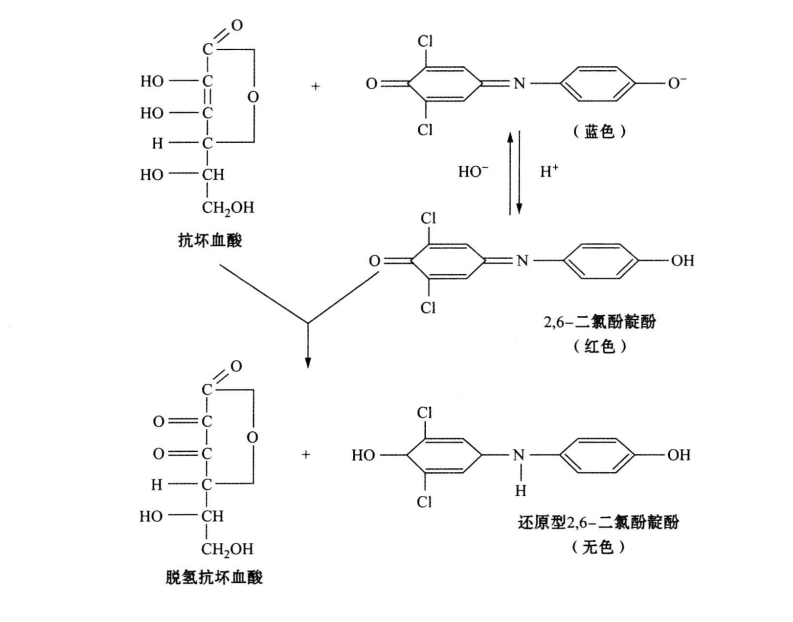
\includegraphics[width=0.8\textwidth]{figures/1.png}
		\caption{2,6-二氯酚靛酚测维生素C含量的原理}
		\label{fig:your_image}
	\end{figure}
	本实验用2,6-二氯酚靛酚作染料,初步测定了维生素C在高温条件下的热稳定性,结果表明,随着温度升高,柑橘中的维生素C含量会不断减少。
该研究为橘子的保存方式与加工方式提供了一定的参考价值。

\section{材料与方法}
\subsection{材料与试剂}
\begin{itemize}
	\item 新鲜橘子若干;
	\item 2\% 草酸溶液:将草酸2g溶于100mL蒸馏水中;
	\item 标准抗坏血酸溶液(1mg/mL):准确称取100mg纯抗坏血酸,溶于1\%草酸溶液并稀释至100mL,贮于棕色瓶中,冷藏;
	\item 0.1\% 2,6-二氯酚靛酚溶液:将250mg 2,6-二氯酚靛酚溶于150mL含有52mgNaHCO3的热水中,冷却后加水稀释至250mL,贮于棕色瓶中冷藏(4°C),约可保存一周。每次临用时,以标准抗坏血酸溶液标定。
\end{itemize}
\subsection{仪器与设备}
锥形瓶100mL;移液管10mL;容量瓶100mL,250mL,50mL;微量滴定管5mL;研钵;漏斗;纱布;恒温水浴锅。
\subsection{试验方法}
将研磨得到的果汁分别在20℃、30℃、40℃、50℃、60°C的温度条件下加热15-20min后,用微量滴定法测定果汁中维生素C的含量,记录滴定消耗2,6-二氯酚靛酚的体积。
\subsection{实验步骤}
\subsubsection{样品的制备}
取一只新鲜橘子,用清水洗净,并用纱布或吸水纸吸干表面水分,然后称取20g,加入20mL2\%草酸,用研钵充分研磨4层纱布过滤,滤液备用。纱布包裹的样品可用少量2\%草酸反复洗几次,合并滤液,滤液总体积定容至50mL。准确吸取滤液五份,每份10mL,分别放入五个50mL锥形瓶内,分别在20℃、30℃、40℃、50℃、60°C的温度条件下恒温加热15-20min。
\subsubsection{标准液滴定}
准确吸取标准抗坏血酸溶液1mL,置于100mL锥形瓶中,加9mL2\%草酸,用微量滴定管以0.1\% 2,6-二氯酚靛酚溶液滴定至淡红色,并保持15s不褪色,即达终点,记录滴定消耗2,6-二氯酚靛酚的体积,由所用染料的体积计算出1mL染料相当于多少毫克抗坏血酸。
\subsubsection{空白对照滴定}
准确吸取2\% 草酸溶液10mL,置于100mL锥形瓶中,用微量滴定管以0.1\% 2,6-二氯酚靛酚溶液滴定至淡红色,并保持15s不褪色,即达终点,记录滴定消耗2,6-二氯酚靛酚的体积。
\subsubsection{样品滴定}
从恒温水浴锅中取出事先放入的10mL样品提取液,用微量滴定管以0.1\% 2,6-二氯酚靛酚溶液滴定至淡红色,并保持15s不褪色,即达终点,记录滴定消耗2,6-二氯酚靛酚的体积。
\subsubsection{维生素的计算}
\[\text{维生素C含量(mg/100g样品)} = \frac{100(V_A - V_B)CT}{DW}\]
式中:\\
$V_A$——滴定样品所耗染料的平均毫升数(mL);\\
$V_B$——滴定空白对照所耗染料的平均毫升数(ml);\\
C——样品提取液的总毫升数(mL);\\
D——滴定时所取的样品提取液毫升数(mL);\\
T——1mL染料能氧化抗坏血酸的毫克数(mg);\\
W——待测样品的重量(g)。\\

\section{实验结果}
\subsection{数据处理}
\begin{table}[H]
	\centering
	\begin{tabular}{ccccc}
		\toprule
		$V_B(ml)$&    $C(ml)$ &      $T(mg)$ & $D(ml)$ &$W(g)$ \\
		\midrule
		0.02 & 50 & 0.4367 & 10 & 20 \\
		\bottomrule
	\end{tabular}
	\caption{原始数据}
\end{table}
\begin{table}[H]
	\centering
	\begin{tabular}{lcc}
		\toprule
		  t(℃)&    $V_A(ml)$ &      维生素含量(mg/100g样品) \\
		\midrule
		 20 &  2.33 &  25.218341 \\
		 30 &  2.31 &  25.000000 \\
		 40 &  2.28 &  24.672489 \\
		 50 &  2.21 &  23.908297 \\
		 60 &  1.98 &  21.397380 \\
		\bottomrule
	\end{tabular}
	\caption{处理后的样品滴定数据}
\end{table}
\subsection{可视化}
\begin{figure}[H]
	\centering
	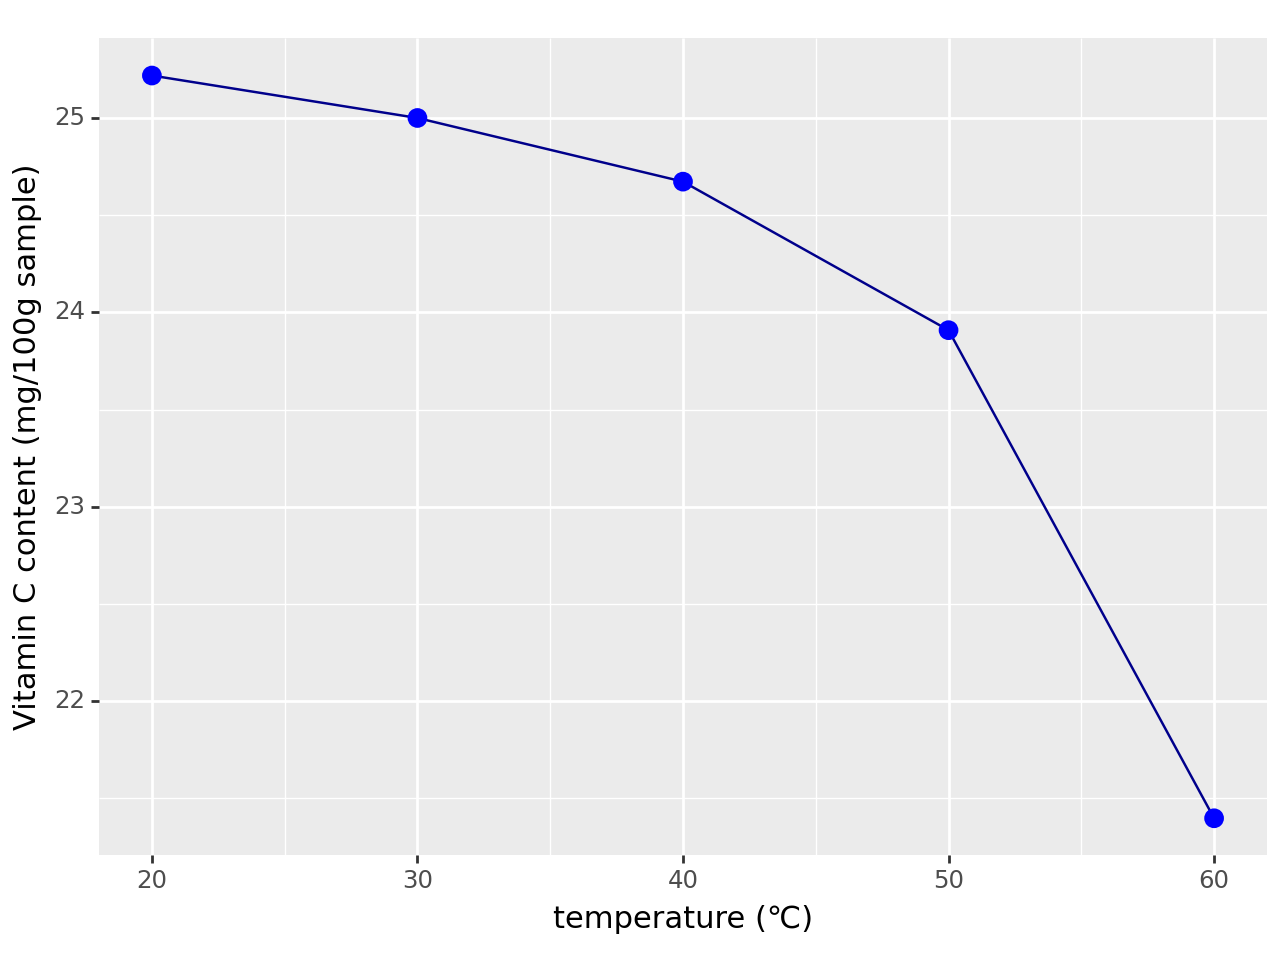
\includegraphics[width=0.8\textwidth]{figures/res.png}
	\caption{橘子中维生素C含量与温度的关系}
	\label{fig:your_image}
\end{figure}
\subsection{结果综述}
常温下,橘子样品中维生素C含量大约为25mg/100g。随着温度升高,测得维生素c含量逐渐升减少;当温度处于50℃以上时,情况尤为明显,维生素C含量显著减少。
\section{讨论与分析}
\subsection{结果分析}
根据美国农业部(USDA)的数据,柑橘(clementine)的平均维生素含量为48.8mg/100g\cite{4},实验测的维生素C含量明显低于标准数据,我认为导致误差很大的原因可能有:
\begin{enumerate}
	\item 没有及时用2\%草酸处理样品,导致维生素C接触到氧气发生氧化反应,导致测量结果偏低;
	\item 本身选取的柑橘已经在实验室存放了比较长时间,在实验之前柑橘果皮已经有干裂,内部的维生素C很可能被氧化了一部分;
	\item 研磨不充分,浆状物中仍有没有完全破碎的柑橘样品;
	\item 维生素C不仅仅存与柑橘的汁囊液体中,果肉、果胶等研磨后不能透过纱布过滤的部分也含有大量维生素C,我认为这是导致误差的主要原因。
\end{enumerate}

从可视化结果上直观来看,随着温度升高柑橘中的维生素C含量不断下降,温度是影响柑橘中维生素C稳定性的重要因素,造成这种现象的原因可能是\cite{5}:
\begin{enumerate}
	\item 维生素C在高温条件下容易分解,我认为这主要是因为维生素分子中含有羟基和醛基,这两个基团很容易发生氧化反应。高温下,氧气的活性增加,加速了维生素C的氧化反应。
		\begin{figure}[H]
		\centering
		
\includegraphics[width=0.25\textwidth]{figures/2.png}
		\caption{维生素C的结构}
		\label{fig:your_image}
	\end{figure}
	\item 从分子碰撞的角度来解释,温度的升高会增加分子的运动速度,使得分子更容易相互碰撞。维生素C的分解反应需要发生碰撞,因此高温下分子碰撞的频率增加,导致维生素C分解的速度加快。
	\item 柑橘中可能存在一些酶,如抗坏血酸氧化酶(AAO)\cite{6},它们在高温下的活性可能增加,加速维生素C的氧化反应,导致维生素C含量下降。
\end{enumerate}
综上所述,温度是影响柑橘中维生素C稳定性的重要因素。较低的温度条件有助于保持维生素C的稳定性,而较高的温度可能导致维生素C的分解或失活。进一步的研究可以探究温度对维生素C稳定性的机制,对于柑橘的储存、运输和加工有着重要意义。

\subsection{实验反思与总结}
本次实验目的是研究不同温度条件对柑橘中维生素C热稳定性的影响。在实验过程中,我们采用滴定法对柑橘样本进行了分析,并根据滴定结果计算了样本中维生素C的含量。以下是我们对实验的反思与总结。

首先,实验结果可能表明温度确实对维生素C的热稳定性产生影响。在高温条件下,样本的维生素C含量可能比低温条件下的样本低,这可能是由于高温加速了维生素C的氧化反应,导致其含量下降。这一结果与我们的预期相符,证实了我们的假设。

然而,实验过程中也存在一些可能的误差来源。例如,滴定过程中的人为误差可能影响了结果的准确性,如滴定液的滴加速度、观察颜色变化的判断等。此外,样本的处理过程中也可能引入误差,如样本的切割、研磨和加热等步骤可能未能严格控制。

总的来说,此次实验为我们提供了宝贵的实践经验,使我们更深入地理解了温度对柑橘中维生素C热稳定性的影响。未来我们将进行更多的实验以进一步验证和深化我们的研究。

在未来的研究中,我们希望能进一步探索其他因素对维生素C热稳定性的影响,如pH值、光照等。同时,我们也希望通过改进实验方法和设备,比如利用高效液相色谱仪来测维生素含量,以减少实验误差,提高实验结果的准确性和可靠性。

%%----------- 参考文献 -------------------%%
%在reference.bib文件中填写参考文献,此处自动生成
\newpage
\section{附页}
\subsection{实验过程图片记录}
\begin{figure}[h]
	\centering
	\subfigure[配置2\%草酸溶液]{
		\includegraphics[width=2.5in]{figures/a1.jpg}
		\label{label_for_cross_ref_1}
	}
	\subfigure[研磨橘子果肉]{
		\includegraphics[width=2.5in]{figures/a2.jpg}
		\label{label_for_cross_ref_2}
	}
	\\    %用 \quad 来换行
	\subfigure[使用4层纱布过滤所得的样品]{
		\includegraphics[width=2.5in]{figures/a3.jpg}
		\label{label_for_cross_ref_1}
	}
	\subfigure[滴定标准抗坏血酸溶液]{
		\includegraphics[width=2.5in]{figures/a4.jpg}
		\label{label_for_cross_ref_2}
	}
	\\ 
	\subfigure[滴定溶液变色]{
		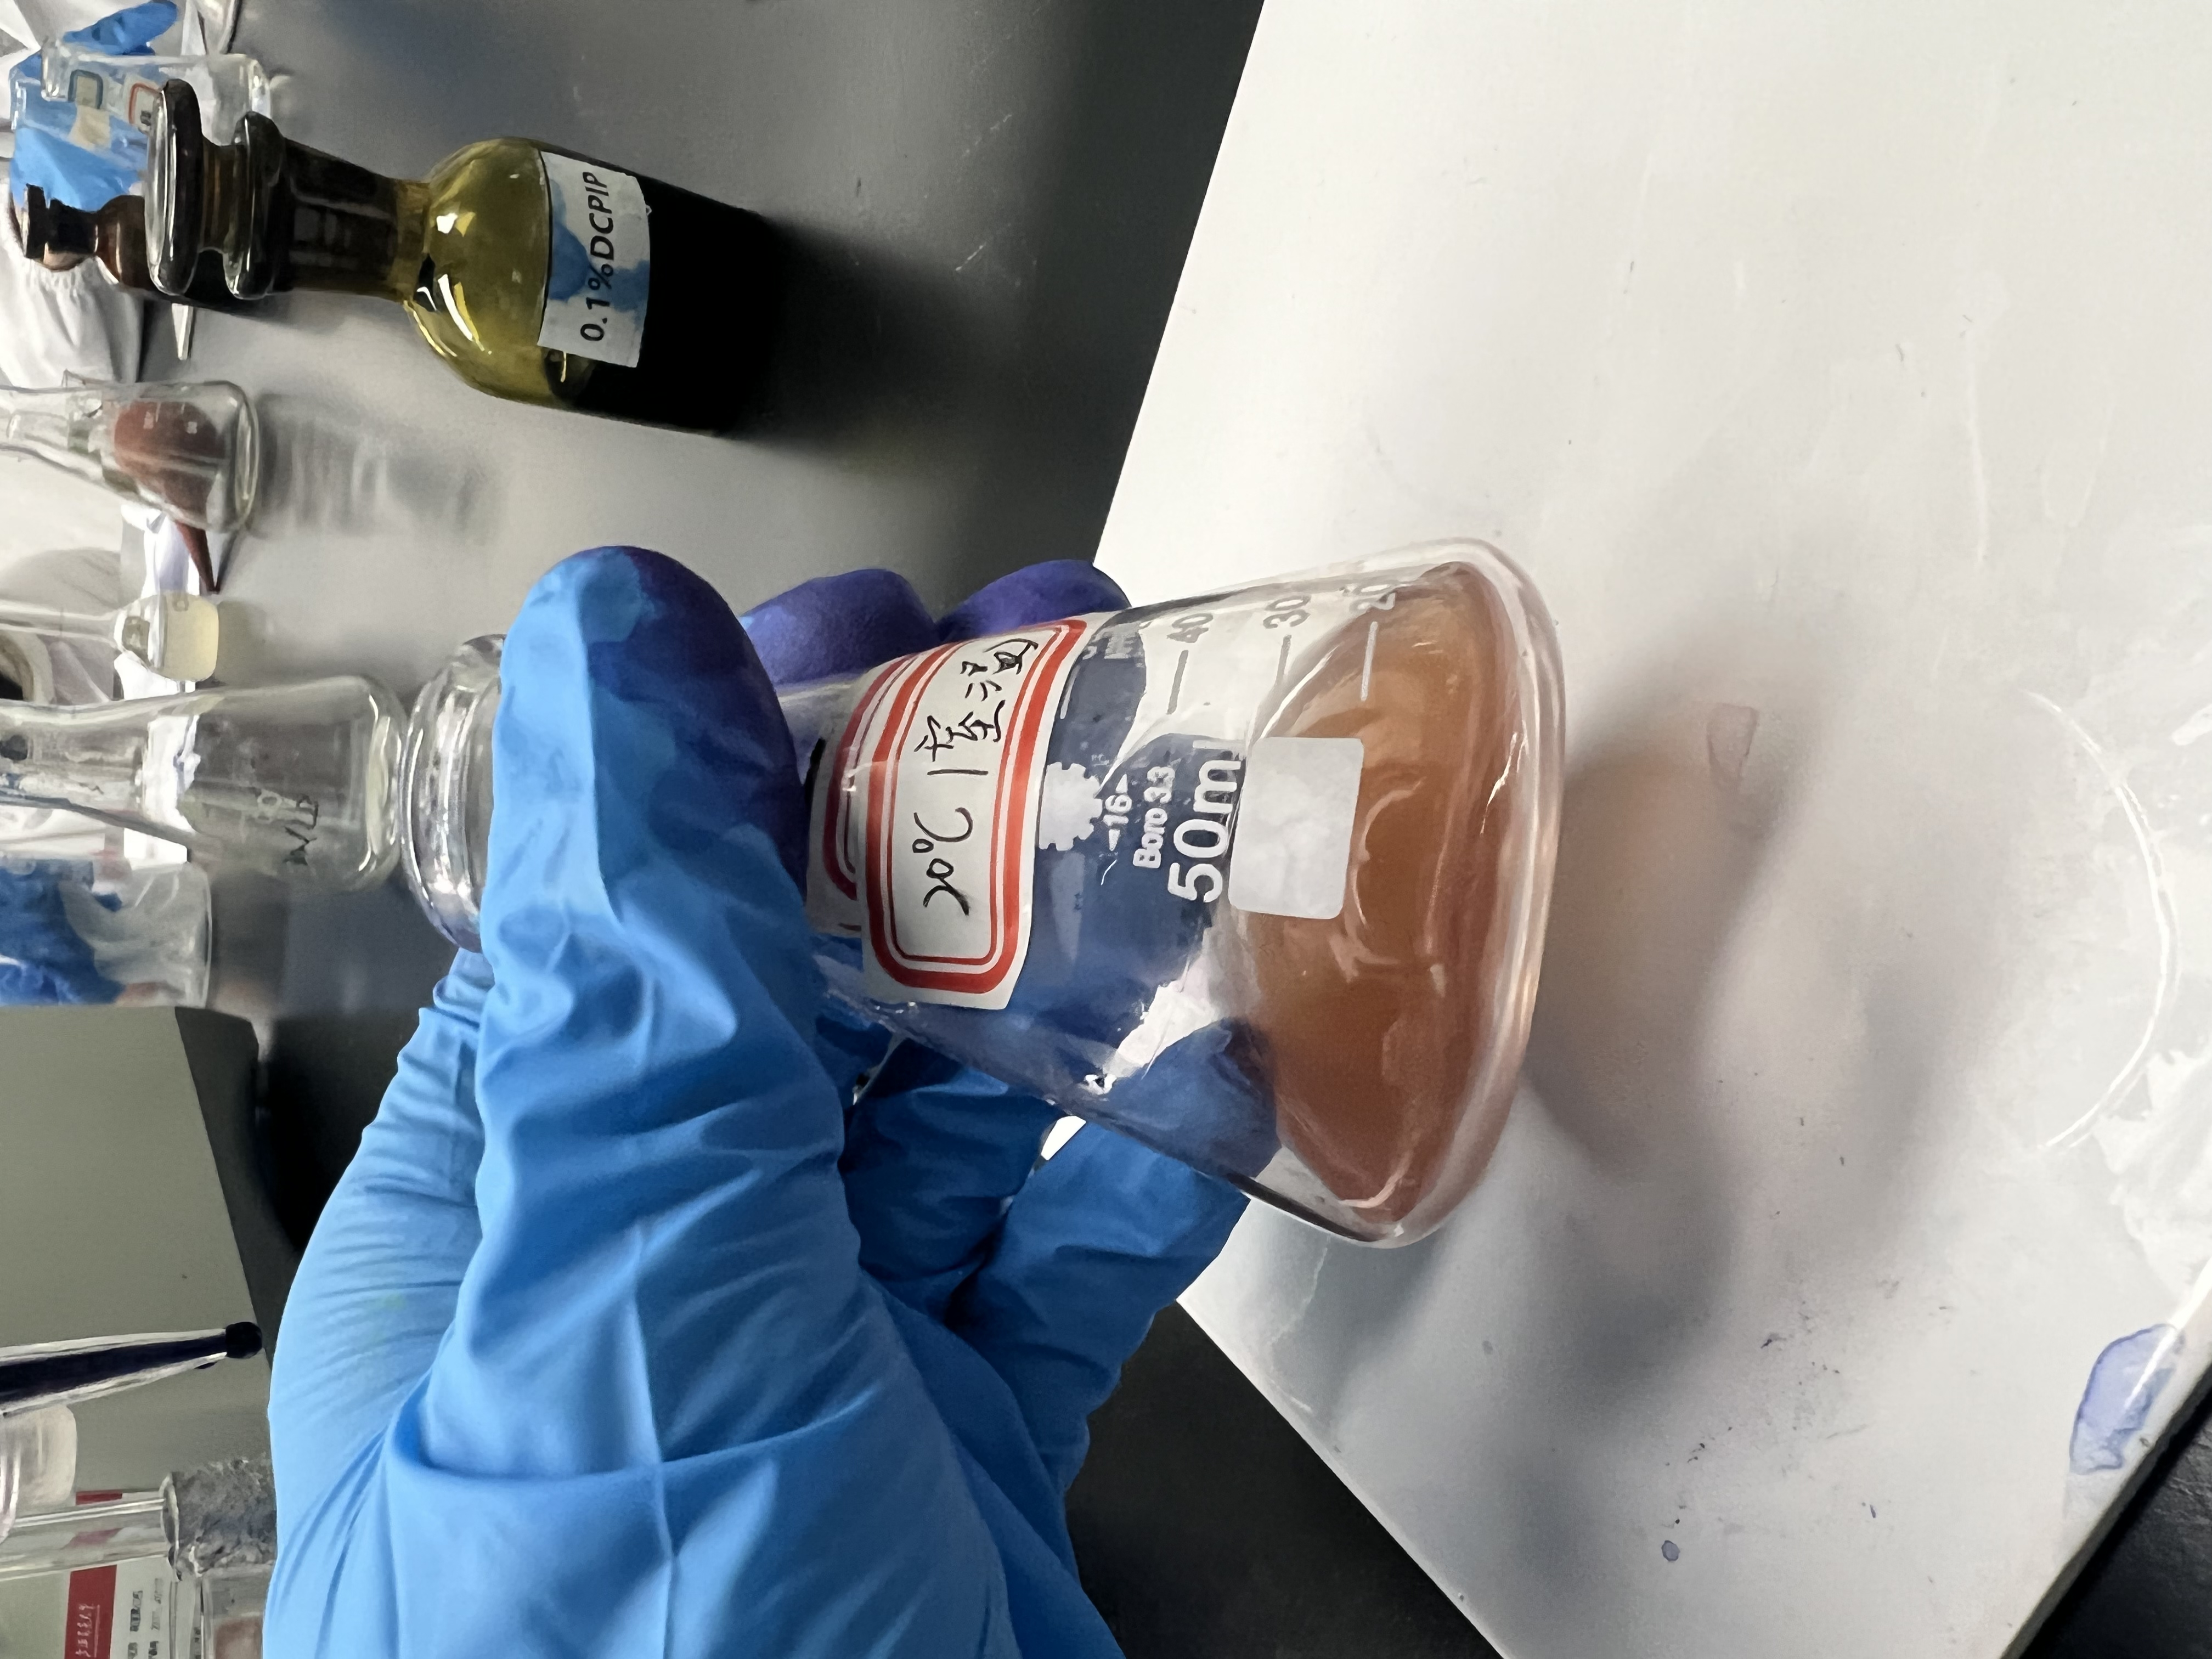
\includegraphics[width=2.5in]{figures/a6.jpg}
		\label{label_for_cross_ref_1}
	}
	\subfigure[滴定不同温度下的样品]{
		\includegraphics[width=2.5in]{figures/a5.jpg}
		\label{label_for_cross_ref_1}
	}
\end{figure}
\newpage
\subsection{数据处理与可视化}
使用python中pandas, numpy和plotnine进行数据分析与可视化,具体代码如下:
\begin{verbatim}
	import pandas as pd
	import numpy as np
	from plotnine import *
	%matplotlib inline
	vb = 0.02
	c = 50
	t = 1/2.29
	d = 10
	w = 20
	df = pd.read_csv('data.csv')
	df['vc'] = 100 * (df['va'] - vb) * c * t / d/ w
	plt = ggplot(df, aes(x = 't', y = 'vc')) + \
	geom_line(color = 'darkblue') + \
	geom_point(size = 3, color = 'blue') + \
	labs(x = 'temperature (℃)', y =  'Vitamin C content (mg/100g sample)')
\end{verbatim}
\reference


\end{document}